\section{{\xtype}: Exception Type Recommender}
\label{sec:xtype}

\begin{figure}[t]
\begin{center}
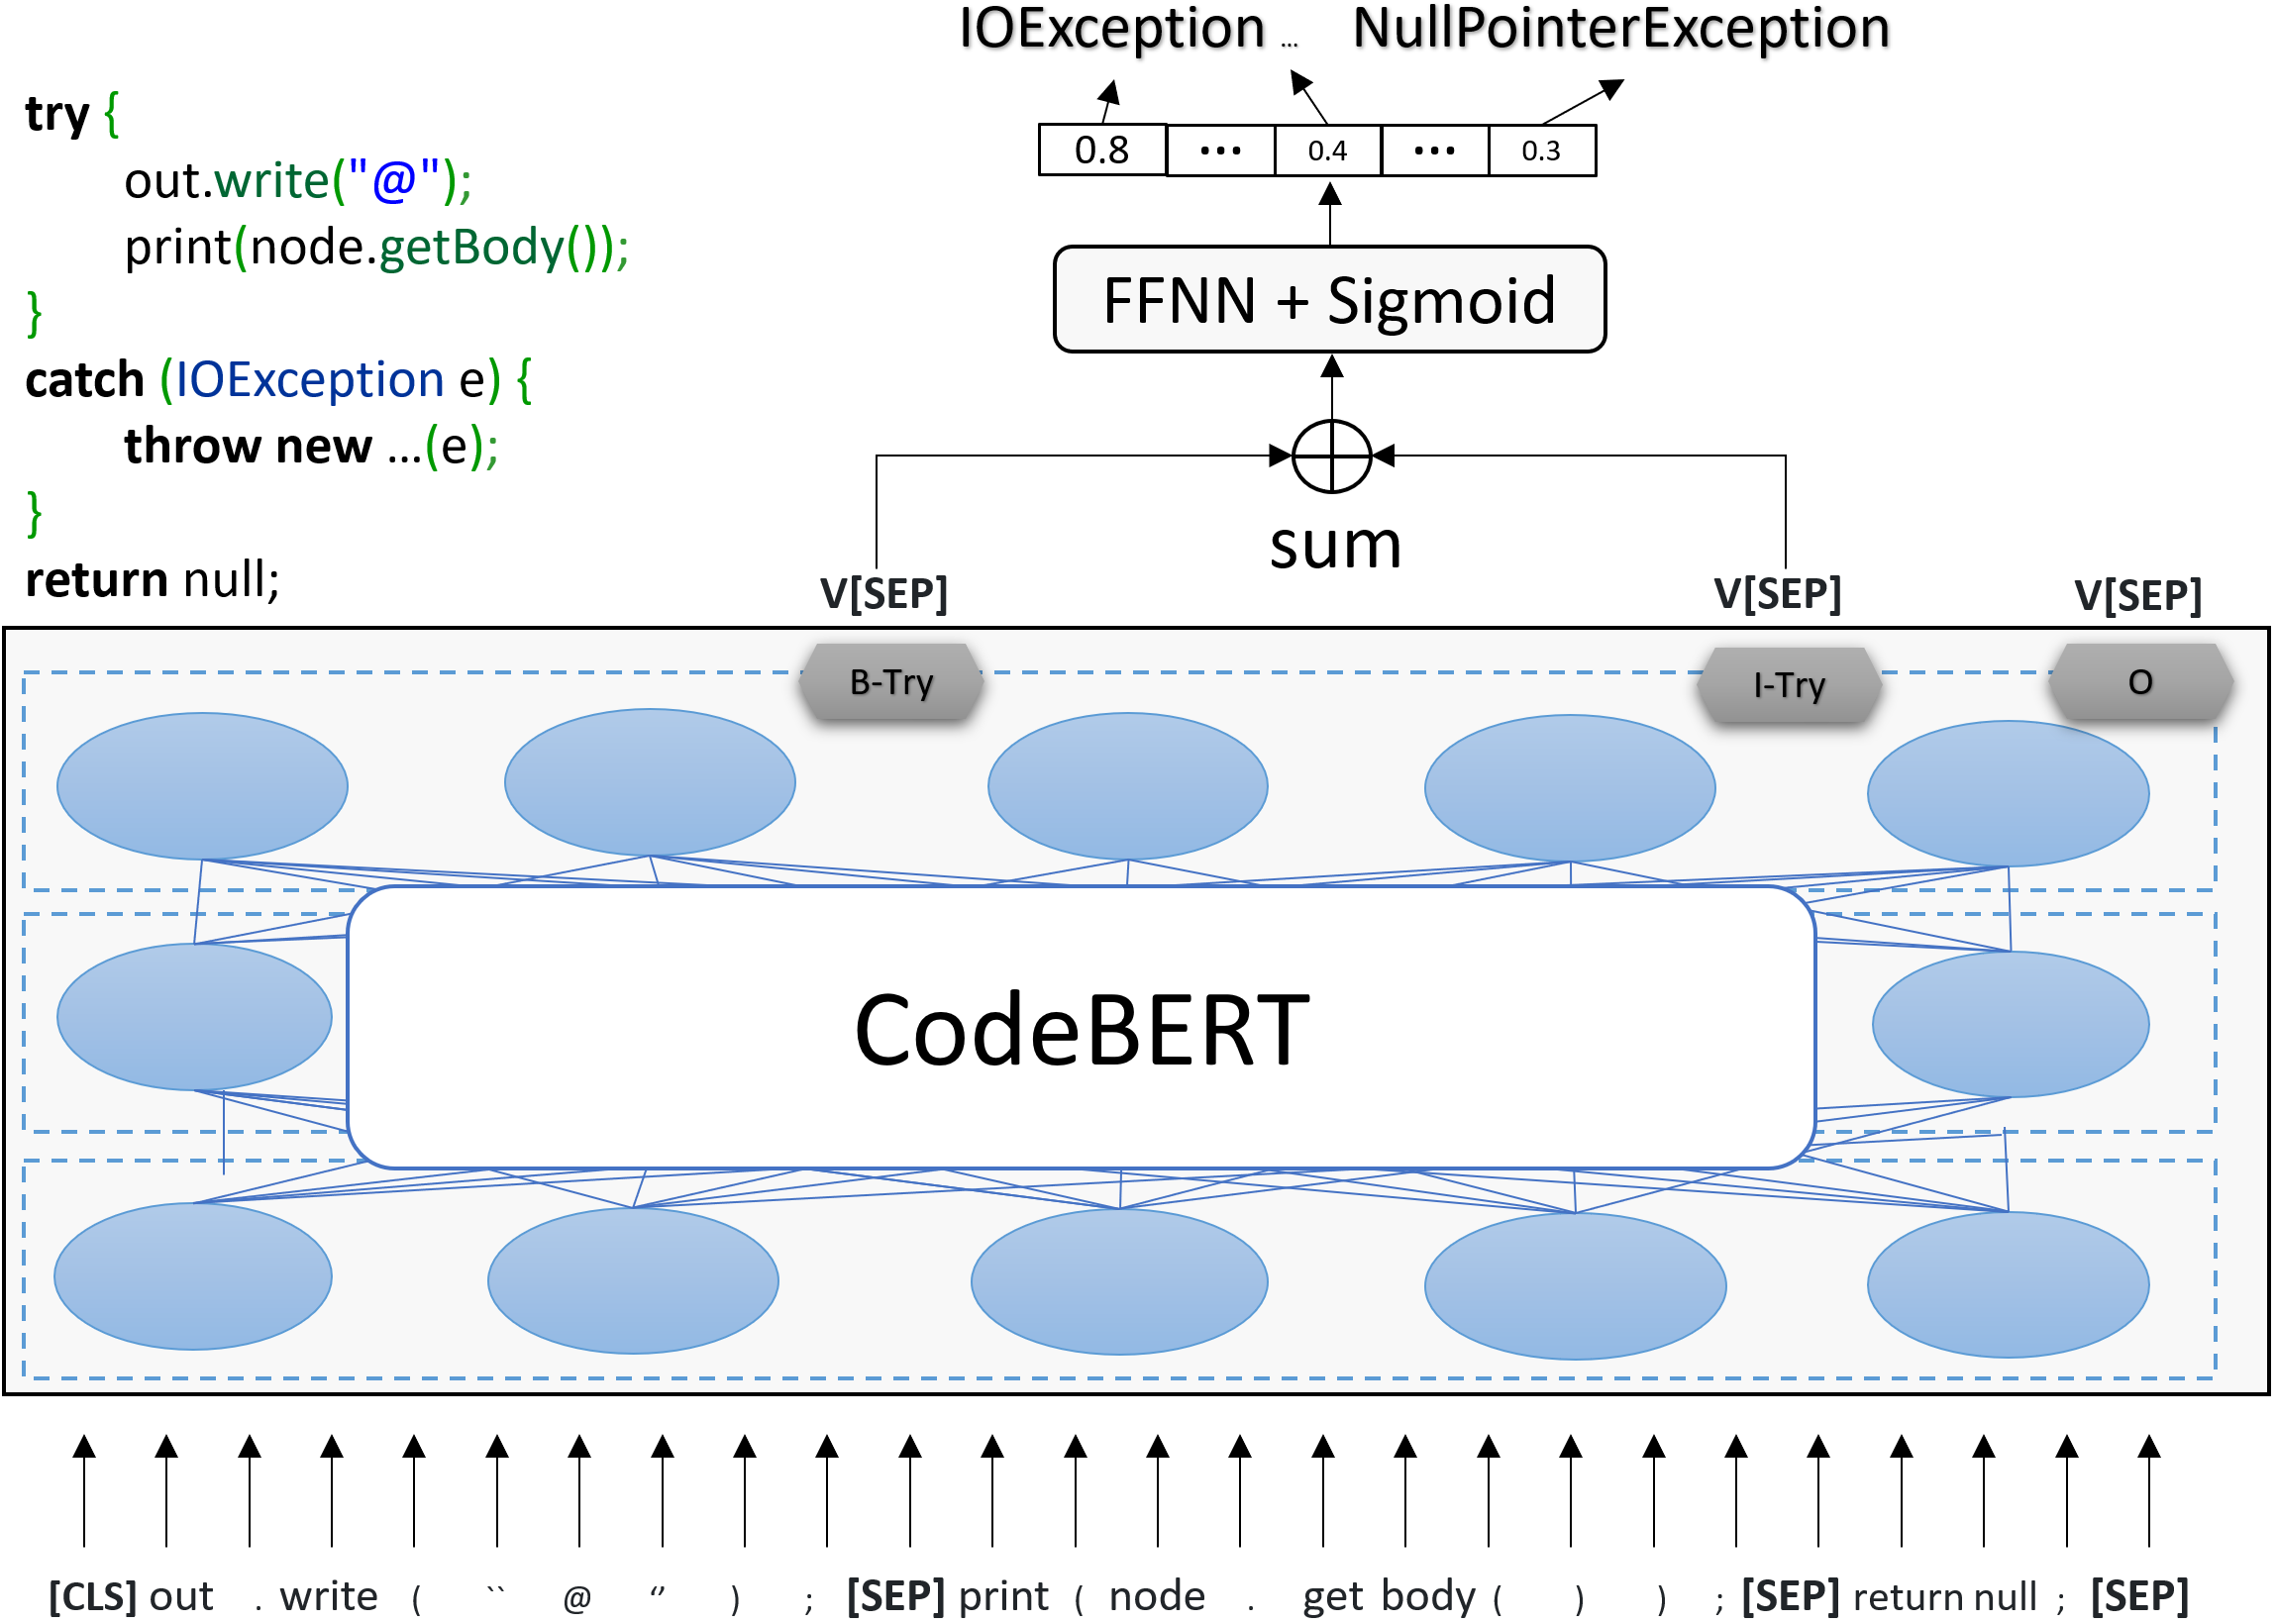
\includegraphics[width=3.2in]{xtype-6.png}
\vspace{-8pt}
\caption{Exception Type Recommendation ({\xtype})}
\label{fig:xtype}
\end{center}
\end{figure}

The goal of {\xtype} (Figure~\ref{fig:xtype}) is to predict what
exception types need to be placed in the \code{catch} clause of each
of the predicted \code{try-catch} block(s) for the given input code
snippet. We use one single CodeBERT~\cite{codebert-emnlp20} model as
in {\xblock} and {\xstate} to build the embeddings for code (sub)-tokens.
%
We expect CodeBERT to learn the connection between the statements in a
\code{try} block and the corresponding exception types to be
caught. From Key Idea 2, we expect that via context, CodeBERT can
implicitly learn the dependencies among API elements, leading to
better learning of the exception~types.

During training, we know all the exceptions to be caught in a code
snippet. For each \code{try} block, we identify the statement
that begins it (with the \code{B-Try} label) and ends it (with the
last respective \code{I-Try} label). Then, we add the embeddings, from
CodeBERT, for the [SEP] tokens that correspond to the statements
inside the \code{try} block and feed this \code{try} block's representation vector into a linear layer.
%We consider the embeddings from CodeBERT for the {\bf [SEP]} tokens
%corresponding to the statements from the beginning to the end of the
%block. We add them together to get the embedding for the entire
%\code{try-catch} block, and feed it into a linear layer.
We use a sigmoid function to perform binary classifications for the
exception types of interest.

During prediction, we use the predicted tags for the given statements
in the code snippet. From the predicted tags, we obtain the the
statements in a predicted \code{try} block. From there, the
embeddings computed by CodeBERT are used in the same way as in
training. For example, in Figure~\ref{fig:xtype}, the model predicts
the \code{try} block from the statement \code{out.write} to the
statement \code{print(node.getBody(...))}. The embeddings of all the
statements in the block are used and the output of \code{IOException}
is predicted since its score is higher than 0.5.
%with the highest probability.



%For each try block, we first take the vector outputs of
%\texttt{[SEP]} tokens, from CodeBERT, that correspond to statements
%in the try block.  If we included more libraries for the study, the
%classification head will likely need to change to a different one.
%During training, we know all the tags associated with every line in
%the input code snippet, so we know how to connect them, while





%\begin{figure}[t]
%\begin{center}
%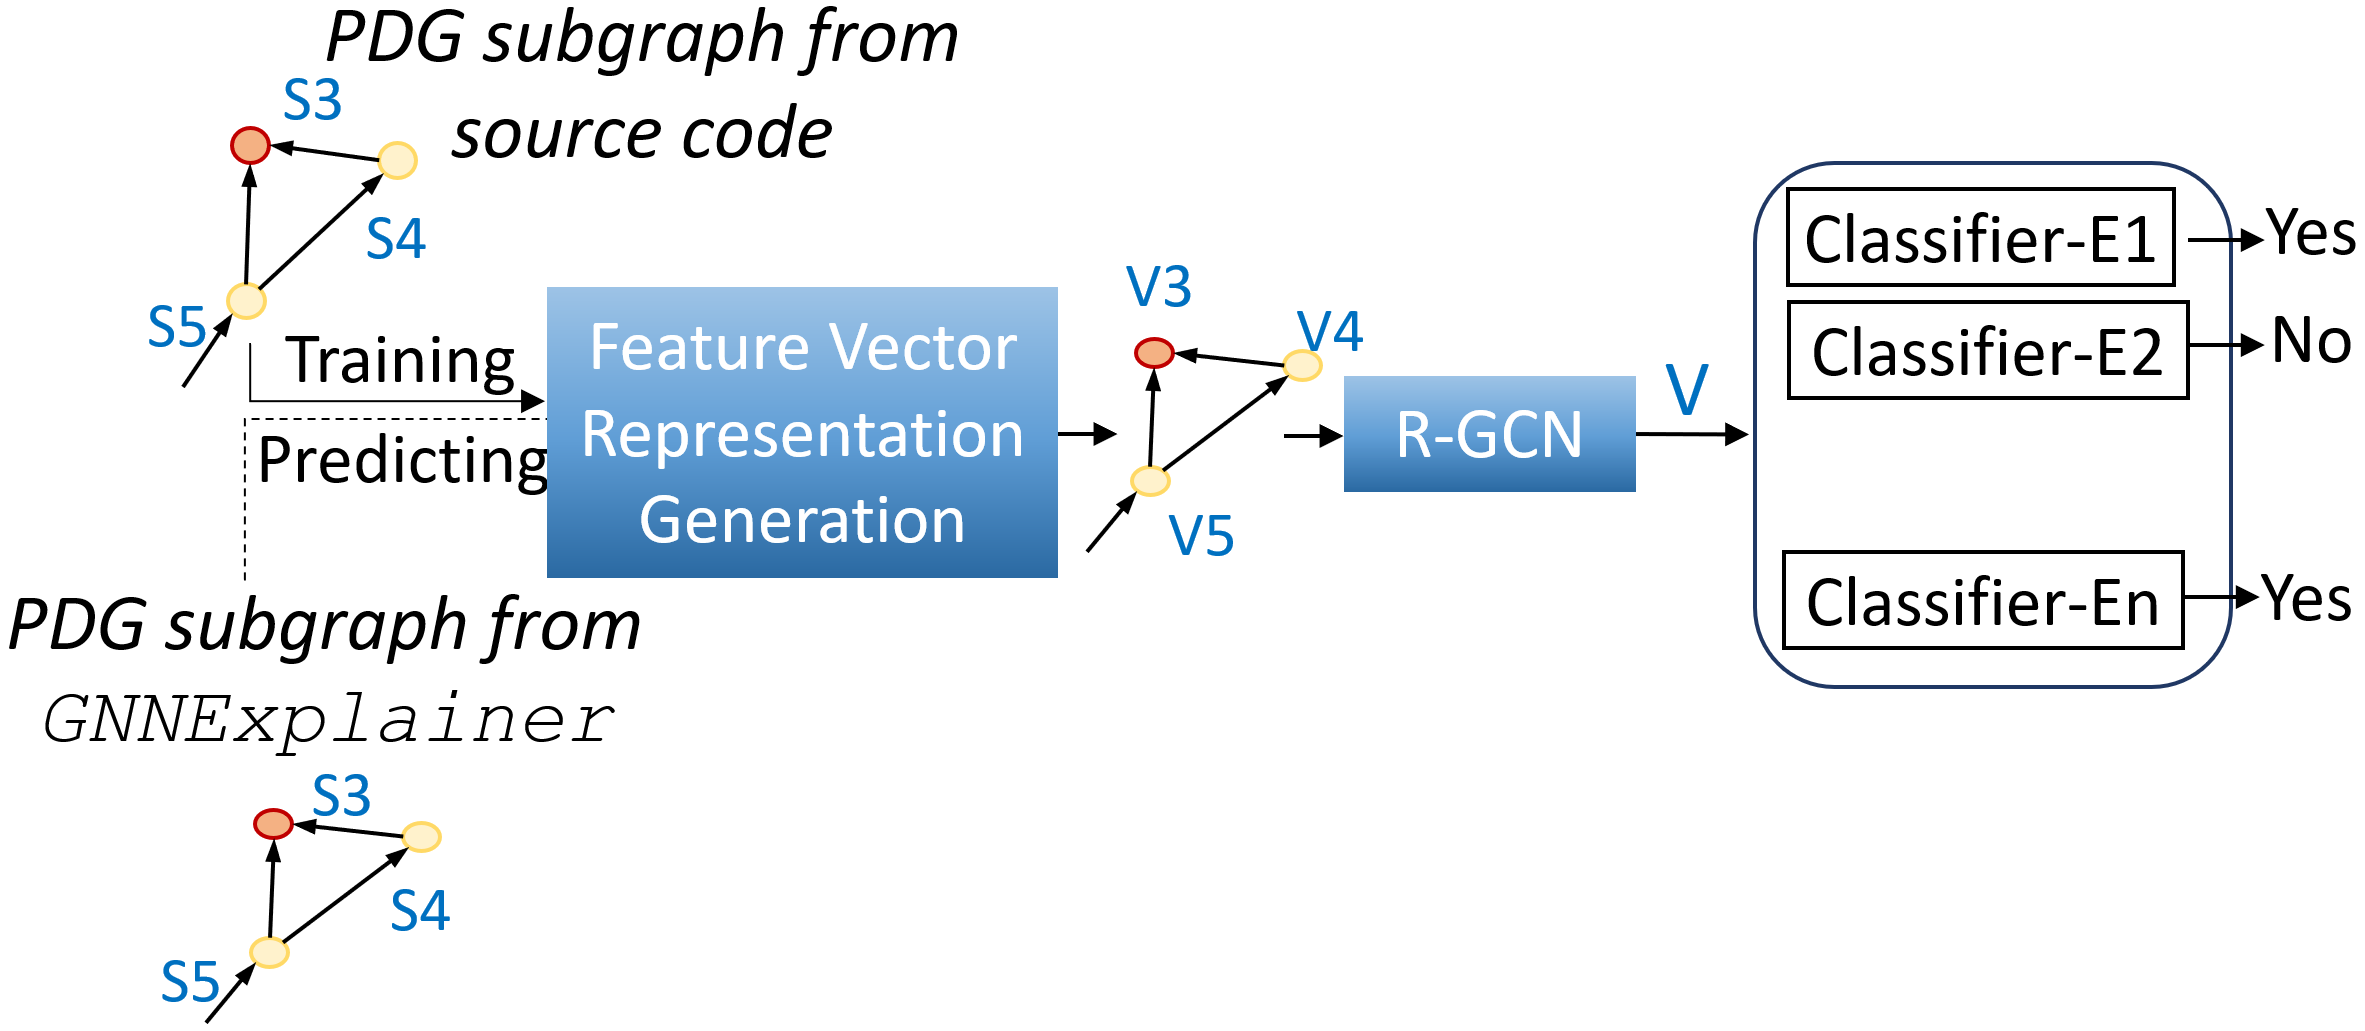
\includegraphics[width=3in]{xtype-3.png}
%\vspace{-10pt}
%\caption{Exception Type Recommendation ({\xtype})}
%\label{fig:xtype}
%\end{center}
%\end{figure}
%
%This section describes {\xtype} that recommends the exception types to
%be handled in the \code{catch} clause for the given code, after the code was
%determined to require a \code{try-catch} block and some of its
%statements were determined to be placed in the \code{try-catch} block.
%
%We use another R-GCN model that acts as a classifier for different
%exception types (Figure~\ref{overview}). For training, the source code
%with \code{try-catch} blocks is used as input. {\tool} parses and
%processes them in the same way to build the PDG subgraph and the
%feature vector representations for the statements as in {\xblock}
%(Figure~\ref{fig:feature}). However, in prediction, the input is the
%sub-graph $\mathcal{G}_C$ of the PDG because the GNNExplainer already
%determined that those statements in that sub-graph need to be placed
%in a \code{try-catch} block. In this case, the feature vectors for the
%sub-graph are also built in the same way as in
%Figure~\ref{fig:feature}. The R-GCN model processes the input
%(sub)graph in a similar manner as in Figure~\ref{fig:gcn} except for the
%processing on the model's output. Instead of connecting
%the output of the R-GCN model to a fully connected layer, we
%feed that output to multiple softmax functions to act as the
%classifiers for the exception types in the dictionary (e.g.,
%\code{IOException}). Each classifier is responsible for one exception
%type.  We could set the maximum number of exception types. The
%positive output from a classifier indicates the presence of the
%corresponding exception type in the \code{catch} clause.
